%!TEX root = /Users/simo/Documents/PFC/Chapter2/chapter2.tex
\section{Comunicación} % (fold)
\label{sec:javascript_comunicacion}
En estos momentos ya es posible renderizar gráficos vectoriales, así como poder dibujarlos de forma interactiva. Es, a efectos prácticos, una \textbf{Pizarra Web}, faltando solo hacerla compartida. Para conseguir esto se han de conseguir dos funcionalidades básicas:

\begin{description}
  \item[Persistencia de los elementos] Es necesario que al crear y eliminar elementos, estos se refleje en una base de datos de fondo, para que en un futuro, estos elementos siguen ahí, y para que el resto de la gente pueda obtener esos elementos.
  \item[Comunicación entre usuarios] Es decir, que los elementos generados por un usuario sean vistos por el otro, de forma automática.
\end{description}

La naturaleza de la web hace esto realmente complicado. El flujo interacción entre un úsuario y una página web es el siguiente:

\begin{figure}[h!]
\centering
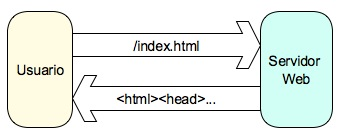
\includegraphics{navigation.png}
\caption{Interacción usuario - servidor}\label{fig:navigation}
\end{figure}

Es un una interacción totalmente pasiva por parte del servidor, el cual solo contesta cuando y si se le solicita un documento. No solo eso, sino que típicamente, la forma de navegar por páginas webs es de ir recargando cada página individualmente. Para este proyecto se necesita algo más, pues la interacción entre el usuario y el servidor tiene que ser totalmente transparente, y por supuesto la página no debe de recargarse cada vez que suceda algún cambio.

En el año 2002, y con el navegador Internet Explorer 5 \footnote{http://es.wikipedia.org/wiki/XMLHttpRequest}, se introdujo la interfaz \texttt{XMLHttpRequest}, que permite abrir conexiones  HTTP con el servidor de forma dinámica mediante Javascript, de forma transparente al usuario, puesto que no necesita recargar la página. Gracias a esto, es posible establecer un flujo de información entre el usuario y el servidor, con el que no solamente transmitir los cambios que dicho usuario haga al documento, sino que permita recibir información de lo que el resto de gente hace.


Las conexiones \texttt{XMLHttpRequest} tienen las mismas características que cualquier otra conexión abierta por un navegador de forma tradicional, con las únicas limitaciones de no poder enviar o recibir archivos de caracter binario. Eso quiere decir que, por ejemplo, es posible pasar parámetros. La diferencia, sin embargo, es que para este tipo de peticiones, no es nada útil que el servidor conteste con documentos que sean páginas web típicas, sino que es necesario que la información sea devuelta en algún formato fácil de entender por un lenguaje de scripting como Javascript. Habitualmente se usa XML, de ahí el nombre de la interfaz, pues es una sintaxis muy adecuada a este tipo de usos, pero es posible recibir cualquier tipo de texto, y de hecho, existen mejores alternativas cuando dicho resultado se va a usar con Javascript. En aplicaciones más modernas se utiliza JSON \footnote{http://es.wikipedia.org/wiki/JSON}, que es básicamente la misma sintaxis utilizada en Javascript para generar objetos (Arrays y Hashes).

\begin{verbatim}
  {
    "page":1,
    "objets": [{"type":"line","x1":10,"x2":20,"y1":0,"y2":5},
               {"type":"circle","x":20,"y":20,"radius":15}]
  }
\end{verbatim}

Ese mismo trozo de código, si se escribiera dentro de una pieza de código Javascript, generaría un Hash con dos atributos, \texttt{page} y \texttt{objects}, y object sería un Array con dos elementos, que a su vez son Hashes. Teniendo ese trozo de texto, en la variable \texttt{response} por ejemplo, que se ha consultado mediante XMLHttpRequest, solo hay que ejecutar la función \texttt{eval} sobre \texttt{response} para generar el objeto correspondiente.

Como era de esperar, la forma de realizar consultas mediante XMLHttpRequest difiere de un navegador a otro, por eso es muy útil utilizar alguna librería, en este caso jQuery, que lo hace tan fácil como usar la función \texttt{get(url)} para consultar una página mediante \texttt{GET}, o \texttt{post(url)} para hacerlo mediante \texttt{POST}.

\begin{verbatim}
  response = $.get("/list_of_elements.json");
  object = eval(response);
  alert(object.page);
\end{verbatim}

Suponiendo que el documento \texttt{list\_of\_elements.json} contiene el trozo de JSON anterior, al realizar un \texttt{alert(object.page)}, se mostrará el valor \textbf{1}.

De la misma forma, se puede utilizar la versión más completa de las funciones para poder enviar información:

\begin{verbatim}
  $.ajax({
    type: "POST",
    url: "/save_circle",
    data: {x: 1, y: 2, radius: 20}
  });
\end{verbatim} 

este comando crearía una solicitud HTTP como la que se genera cuando se rellena un formulario, mandándola mediante POST, con los atributos especificados en data. Lógicamente es necesario un sistema que sea capaz de entender todas estas solicitudes, pero por ahora este capítulo se centrará en como el Javascript tratará todas las comunicaciones necesarios con el servidor, suponiendo siempre que existe el sistema que actuará de forma adecuada.

\newpage
\subsection{Crear y destruir elementos} % (fold)
\label{ssub:crear_y_destruir_elementos}

Esta parte es la más sencilla, puesto que solo es necesario comunicar al servidor de los cambios realizados por el usuario en concreto. En todos los casos está muy claro cuando se crea un elemento, y cuando se elimina, por tanto, ese será el momento de comunicarlo. 

El primer problemaes decidir de qué forma se va a representar un elemento. Recordando que cada elemento tiene atributos diferentes, y que todo ha de acabar siendo almacenado en una base de datos relacional, es posible que todo pueda llegar a complicarse. Lo más sencillo en este caso sería que todos los elementos, sean del tipo que sean, pudieran ser guardados en una misma tabla de una base de datos, y que por tanto, tubieran los mismos atributos.

Puesto que siempre que se consulten datos al servidor, éste los comunicará en forma de JSON, se ha creído adecuado que ocurra el mismo proceso en sentido inverso. La forma de que todos los objetos puedan estar en la misma tabla, es codificándolos de alguna manera de forma que puedan representarse mediante una cadena de texto. De la misma forma que, con una cadena de texto en formato JSON es posible generar un objeto en Javascript, es posible realizar el proceso opuesto. Suponiendo la existencia de una función \texttt{toJSON(object)} que devuelva un string representativo del objeto, el proceso para comunicar al servidor un nuevo elemento, podría ser el siguiente:

\begin{verbatim}
  function save(it){
  	var text = toJSON(it);
  	$.ajax({
  		url: "/add_element",
  		data: {attr: text}
  	});
  }
\end{verbatim}

Ésta es una versión simplificada de la función que se ha acabado usando en realidad, pero ya sirve para ver el proceso que se ha seguido. Es necesario añadir una serie de mejoras, que se comentan a continuación.

¿Cómo sabe el sistema a qué documento pertenece este elemento? Es necesario enviar información para que se sepa a qué documento corresponde este elemento. Puesto que habrá una base de datos de fondo, es posible suponer que siempre habrá un identificador para documento, y que es conocido de alguna manera por el javascript, pues se habrá definido al cargar la página.

\begin{verbatim}
  function save(it){
  	var text = toJSON(it);
  	$.ajax({
  		url: "/add_element",
  		data: {attr: text, :doc: docId}
  	});
  }
\end{verbatim}

La parte de crear elemento se puede considerar como resuelta. En cuanto eliminar objetos, es necesario saber algo más. ¿Cómo se le comunica al sistema qué elemento se ha eliminado? De la misma forma, es posible suponer que en la base de datos, estos objetos tendrán asignado un identificador como clave primaria. Este identificador se genera al crear dicho elemento, por lo tanto no es posible saberlo hasta que no se ha comunicado al servidor. La solución para esto es modificar la función de guardado de elementos, haciendo que el servidor conteste a la consulta que agrega un elemento, con el id generado para dicho elemento. Aunque una consulta se utilice para transmitir información, el servidor siempre debe contestar algo, por lo tanto es posible aprovechar estos datos:

\begin{verbatim}
  function save(it){
  	var text = toJSON(it);
  	$.ajax({
  	  url: "/add_element",
  	  data: {attr: text, :doc: docId},
  	  success: function(ret){
  	    it.element.id=ret;
  	  }
  	});
  }
\end{verbatim}

Este cambio agrega código personalizado al evento success de esta consulta XMLHttpRequest. jQuery lanza eventos en diferentes puntos de las consultas para que el programador pueda ejecutar distintas acciones en los distintos puntos de la consulta. Los eventos generados son \texttt{beforeSend, complete, success} y \texttt{error}, todos ellos suficientemente descriptivos.

En este caso, cuando la consulta finaliza y es satisfactoria, y suponiendo que el servidor ha contestado simplemente con el id del elemento creado, se coge el objeto que se había guardado, y se modifica añadiéndole un campo id con dicho valor. De esta forma, los elementos representados en pantalla tienen el id correspondiente a su equivalente de la base de datos, y permiten, por tanto, simplificar la función de borrado a un simple:

\begin{verbatim}
  //IE
  $.get("/remove_element/" + event.srcElement.id);
  //RESTO
  $.get("/remove_element/" + event.target.id);
\end{verbatim}

utilizando, como ya se había comentado anteriormente, los atributos \texttt{srcElement} y \texttt{target} de la \textbf{variable de estado}, para saber con qué elementos se estaba tratando.

% subsubsection crear_y_destruir_elementos (end)
\newpage
\subsection{Sincronización entre usuarios} % (fold)
\label{ssub:sincronizacion_entre_usuarios}

Uno de los mayores retos a los que se enfrenta esta aplicación, es mantener a todos los usuarios sincronizados. Hasta este momento es posible mantener al servidor informado de la creación y eliminación de elementos, pero no es posible informar al resto de usuarios de dichas acciones. En el caso de aplicaciónes típicas, con un paradigma cliente-servidor en que el servidor pudiera iniciar transferencias de información, lo lógico sería que cuando hubiera algún cambio, el servidor informara al resto de clientes de los cambios.

Sin embargo, en el caso de una página web, esto no es posible. No hay ninguna posibilidad de que el servidor establezca una conexión con el usuario por iniciativa propia, y por tanto la única solución restante es realizar consultas periódicas en busca de nuevos cambios. El tiempo entre consulta y consulta, así como la latencia entre el servidor y el cliente, son los factores que definen el tiempo entre que se realiza un cambio y el momento en que el resto de usuarios es consciente de ello.

Teniendo en cuenta que la latencia es un parámetro incontrolable, la única posibilidad para mejorar los tiempos es cambiar el tiempo entre una consulta y otra. Existen dos estrategias posibles para esto, ambas perfectamente viables, aunque adecuadas para diferentes necesidades.

\subsubsection{Realizar peticiones cada periodo de tiempo fijo} % (fold)
\label{ssub:nunca_tener_más_de_una_petición_pendiente}
El enfoque más directo y más logico en un primer acercamiento al problema, es ir lanzando peticiones periódicamente, sin importar que peticiones anteriores hayan sido contestadas ya o no. Suponiendo una latencia de unos 200ms entre servidor y usuario, el tiempo de estabilidad $t_e$ será de $ 2t_l < t_e > 2t_l + t_r$ con $t_l$ siendo la latencia y $t_r$ el tiempo entre peticiones. Este enfoque permite personalizar al máximo el comportamiento de la aplicación, pudiendo tener mejores tiempos si se dispone de recursos suficientes, o empeorándolos en caso contrario.

Sin embargo, este enfoque produce una serie de problemas asociados al hecho de tener conexiones simultáneas pendientes. Debido a que la latencia no es un número fijo, y por tanto es posible completar peticiones en orden distinto al que se han generado, se debería realizar todo un control de paquetes semejante al realizado por TCP en las redes de datos, para permitir un comportamiento adecuado de la aplicación.

\begin{quotation}
  Un elemento es creado en momento $0$ por el usuario $u1$. El servidor, debido a la latencia, recibe notificación del cambio en el momento $10$. Mientras tanto, el usuario $u2$, ha ido mandando peticiones cada unidad de tiempo, pero debido a la inestabilidad de la red, recibe primero el resultado de una petición que llegó al servidor en el momento $11$, antes que otra que había llegado al servidor en el momento $9$. Debido a ello, primero recibe notificación de borrar el elemento, puesto que ya no está, y después la segunda notificación le informa de que aún sigue ahí.
\end{quotation}

Este es solo el primero de varios problemas posible, sin tener en cuenta que varios usuarios pueden agregar o eliminar elementos al mismo tiempo, cambiar de página, o que el servidor se caiga y se deje de recibir contestaciones. No es, ni mucho menos, una tarea imposible de realizar, pero si requiere de un grado de control extra.

% subsubsection nunca_tener_más_de_una_petición_pendiente (end)

\subsubsection{Una petición a la vez} % (fold)
\label{ssub:una_peticion_a_la_vez}
Otro enfoque posible es el de ir realizando peticiones contínuas, pero siempre una detrás de otra. Es decir, generando la petición, procesando la respuesta, y generando una petición inmediatamente después. Con este planteamiento es posible ignorar la mayoría de problemas de sincronización comentados, y permitirá una menor carga por parte tanto del servidor como del navegador del usuario. El tiempo de estabilidad en este caso, sería de $ 2t_l < t_e > 4t_l$ . De nuevo, tomando una latencia media de 200ms, se baraja un $t_e$ de casi un segundo.

Comparando con la estrategia anterior, sin embargo, se puede observar que esta diferencia no es tan acentuada. Un planteamento realista no contemplaría más de cuatro o cinco peticiones por segundo, en cuyo caso se estaría hablando de nuevo, de un $t_r$ de 200ms, con lo cual se estaría en un $t_e$ entre 400ms y 600ms (500ms de media). Comparado con esta segunda estrategia, en la cual se maneja un $t_e$ de entre 400 y 800ms (600ms de media), solo se obtendría un beneficio de unos 100ms de media, además de reducir de $5$ peticiones por segundo a $2,5$.

Con una diferencia tan pequeña, no se considera necesario el esfuerzo necesario para mantener un sistema con el primer enfoque, y que el segundo, siendo más sencillo y robusto, permitirá una mayor fiabilidad del código.

% subsubsection una_peticion_a_la_vez (end)

% subsubsection sincronización_entre_usuarios (end)

% section javascript_comunicacion (end)